\documentclass[20pt]{article}

\usepackage{geometry}
\usepackage{titlesec}
\usepackage{amsmath}
\usepackage{amssymb}
\usepackage{times}
\usepackage{tipa}
\usepackage{covington}
\usepackage{tikz}
\usepackage{tikz-qtree}

\setlength\parindent{0pt}
\newcommand{\ipa}[1]{\textipa{#1}}
\newcommand{\broad}[1]{/\ipa{#1}/}
\newcommand{\narrow}[1]{[ \ipa{#1} ]}
\newcommand{\english}[1]{$<$#1$>$}
\newcommand{\sk}[0]{{\kern 0.05em}}
\newcommand{\mk}[0]{{\kern 0.1em}}
\newcommand{\smallcapi}[0]{\sk\textsci\sk}
\newcommand{\openo}[0]{\sk O}
\newcommand{\feature}[1]{\ensuremath{\left[ \text{#1} \right]}}
\newcommand{\treeScale}[0]{0.9}
\newcommand{\rolesOpacity}[0]{0.7}
\newcommand{\rolesOne}[0]{$<$$\theta$$>$}
\newcommand{\rolesTwo}[0]{$<$$\theta$,$\theta$$>$}
\newcommand{\rolesThree}[0]{$<$$\theta$,$\theta$,$\theta$$>$}
\newcommand{\constituent}[2]{$[_{\text{#1}}$ #2$]$}
\definecolor{darkgreen}{HTML}{006400}

\titlespacing*{\section}{0pt}{0.7\baselineskip}{0.7\baselineskip}
\titleformat*{\section}{\large\bfseries}

\begin{document}

\Large\textbf{Problem Set 6} \\
\normalsize
Alice McKean \\
\today

\section{Tree Structures, Theta Roles, and Case Assignment}

In the following trees \textcolor{blue}{blue} depicts theta role assignment,
\textcolor{red}{red} depicts accusative case assignment, and
\textcolor{darkgreen}{green} depicts nominative case assignment. \\

\begin{tikzpicture}[scale=\treeScale, transform shape]
  \tikzset{every tree node/.style={align=center,anchor=north}}
  \Tree
  [.TP
    [.\node(DP-1-1){DP};
      D\\\feature{PROP}
      NP\\Alix
    ]
    [.T'
      \node(T-1){T\\\feature{PAST}};
      [.VP
        \node(V-1){V\\tried\\\rolesTwo};
        [.\node(CP-1-1){CP};
          C\\$\emptyset$
          [.TP
            \node(DP-2-1){DP\\\feature{PRO}};
            [.T'
              T\\to
              [.VP
                [.VP
                  \node(V-2){V\\finish\\\rolesTwo};
                  [.\node(DP-2-2){DP};
                    D\\the
                    NP\\report
                  ]
                ]
                [.PP
                  \node(P-2-1){P\\before\\\rolesOne};
                  [.\node(CP-2-1){CP};
                    C\\$\emptyset$
                    [.TP
                      [.\node(DP-3-1){DP};
                        D\\the
                        NP\\boss
                      ]
                      [.T'
                        \node(T-3){T\\\feature{PAST}};
                        \node(V-3){VP\\returned\\\rolesOne};
                      ]
                    ]
                  ]
                ]
              ]
            ]
          ]
        ]
      ]
    ]
  ]
  \draw[blue, opacity=\rolesOpacity, ->] (V-1) -- (DP-1-1);
  \draw[blue, opacity=\rolesOpacity, ->] (V-1) -- (CP-1-1);
  \draw[blue, opacity=\rolesOpacity, ->] (V-2) -- (DP-2-1);
  \draw[blue, opacity=\rolesOpacity, ->] (V-2) -- (DP-2-2);
  \draw[blue, opacity=\rolesOpacity, ->] (P-2-1) -- (CP-2-1);
  \draw[blue, opacity=\rolesOpacity, ->] (V-3) -- (DP-3-1);
  \draw[darkgreen, opacity=\rolesOpacity, ->] ([yshift=20pt]T-1) -- (DP-1-1);
  \draw[darkgreen, opacity=\rolesOpacity, ->] ([yshift=-10pt]T-3) -- (DP-3-1);
  \draw[red, opacity=\rolesOpacity, ->] ([yshift=-20pt]V-2) -- (DP-2-2);
\end{tikzpicture} \\

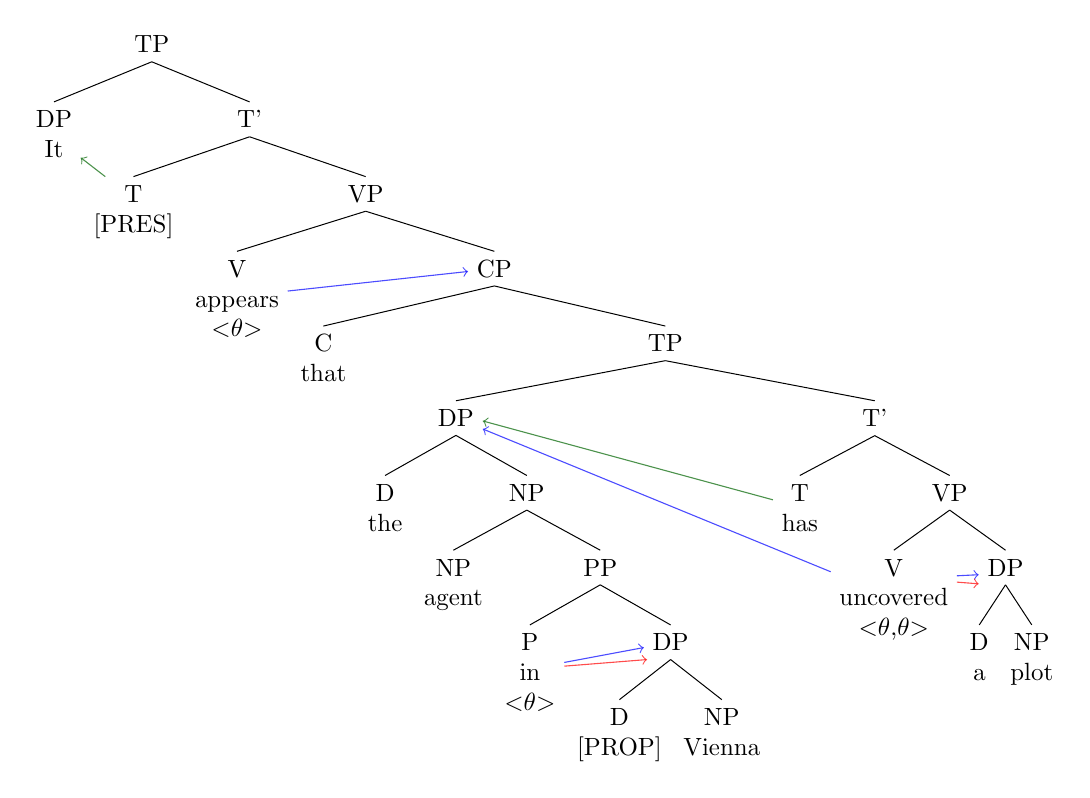
\begin{tikzpicture}[scale=\treeScale, transform shape]
  \tikzset{every tree node/.style={align=center,anchor=north}}
  \Tree
  [.TP
    \node(DP-1-1){DP\\{It}};
    [.T'
      \node(T-1){T\\\feature{PRES}};
      [.VP
        \node(V-1){V\\appears\\\rolesOne};
        [.\node(CP-1-1){CP};
          C\\that
          [.TP
            [.\node(DP-2-1){DP};
              D\\the
              [.NP
                NP\\agent
                [.PP
                  \node(P-2-1){P\\in\\\rolesOne};
                  [.\node(DP-2-2){DP};
                    D\\\feature{PROP}
                    NP\\Vienna
                  ]
                ]
              ]
            ]
            [.T'
              \node(T-2){T\\has};
              [.VP
                \node(V-2){V\\uncovered\\\rolesTwo};
                [.\node(DP-2-3){DP};
                  D\\a
                  NP\\plot
                ]
              ]
            ]
          ]
        ]
      ]
    ]
  ] 
  \draw[blue, opacity=\rolesOpacity, ->] (V-1) -- (CP-1-1);
  \draw[blue, opacity=\rolesOpacity, ->] (P-2-1) -- (DP-2-2);
  \draw[blue, opacity=\rolesOpacity, ->] (V-2) -- (DP-2-1);
  \draw[blue, opacity=\rolesOpacity, ->] (V-2) -- (DP-2-3);
  \draw[red, opacity=\rolesOpacity, ->] ([yshift=-30pt]P-2-1) -- (DP-2-2);
  \draw[red, opacity=\rolesOpacity, ->] ([yshift=-15pt]V-2) -- (DP-2-3);
  \draw[darkgreen, opacity=\rolesOpacity, ->] (T-1) -- (DP-1-1);
  \draw[darkgreen, opacity=\rolesOpacity, ->] ([yshift=20pt]T-2) -- (DP-2-1);
\end{tikzpicture} \\

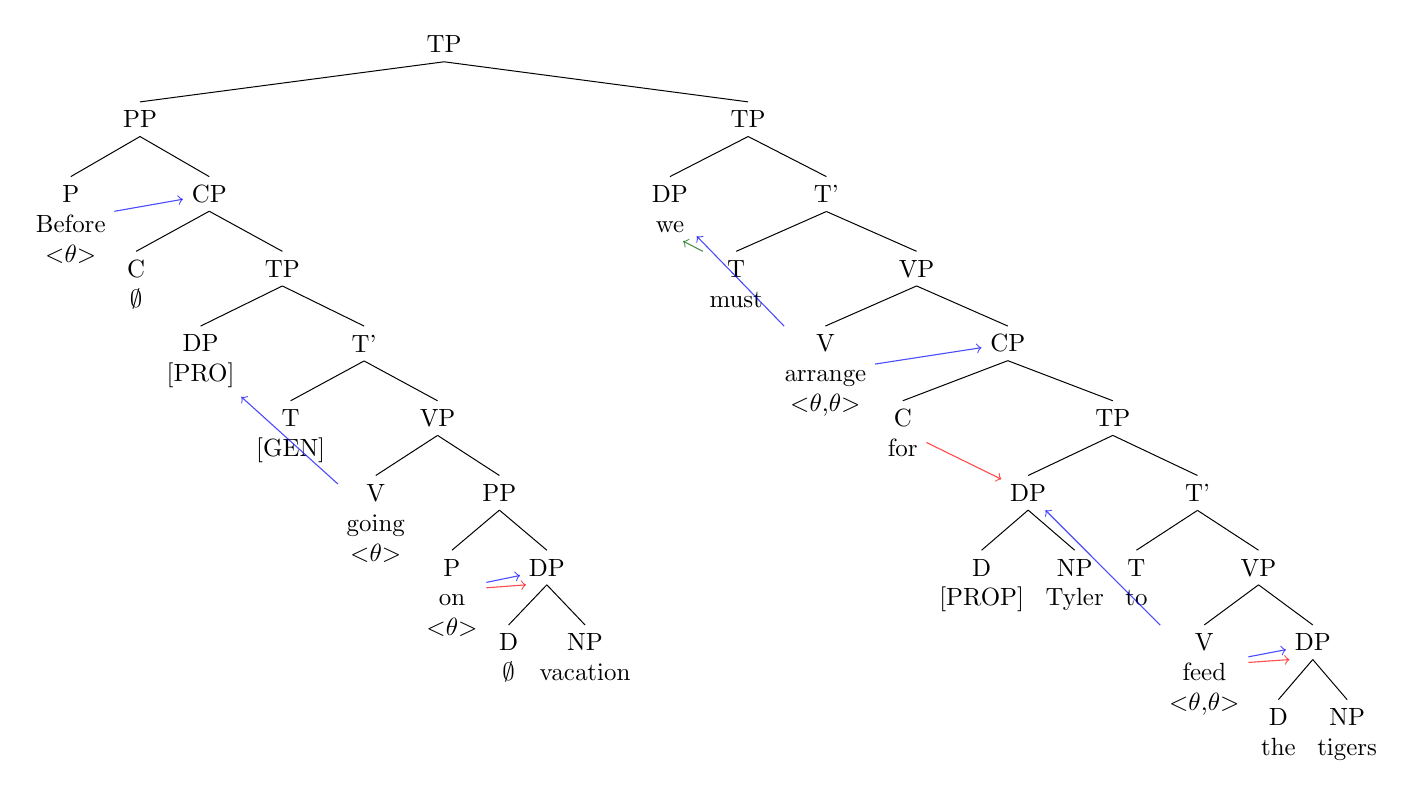
\begin{tikzpicture}[scale=\treeScale, transform shape]
  \tikzset{every tree node/.style={align=center,anchor=north}}
  \Tree
  [.TP
    [.PP
      \node(P-1-1){P\\Before\\\rolesOne};
      [.\node(CP-1-1){CP};
        C\\$\emptyset$
        [.TP
          \node(DP-2-1){DP\\\feature{PRO}};
          [.T'
            T\\\feature{GEN}
            [.VP
              \node(V-2){V\\going\\\rolesOne};
              [.PP
                \node(P-2-1){P\\on\\\rolesOne};
                [.\node(DP-2-2){DP};
                  D\\$\emptyset$
                  NP\\vacation
                ]
              ]
            ]
          ]
        ]
      ]
    ]
    [.TP
      \node(DP-3-1){DP\\we};
      [.T'
        \node(T-3){T\\must};
        [.VP
          \node(V-3){V\\arrange\\\rolesTwo};
          [.\node(CP-3-1){CP};
            \node(C-3-1){C\\for};
            [.TP
              [.\node(DP-4-1){DP};
                D\\\feature{PROP}
                NP\\Tyler
              ]
              [.T'
                T\\to
                [.VP
                  \node(V-4){V\\feed\\\rolesTwo};
                  [.\node(DP-4-2){DP};
                    D\\the
                    NP\\tigers
                  ]
                ]
              ]
            ]
          ]
        ]
      ]
    ]
  ]
  \draw[blue, opacity=\rolesOpacity, ->] (P-1-1) -- (CP-1-1);
  \draw[blue, opacity=\rolesOpacity, ->] (V-2) -- (DP-2-1);
  \draw[blue, opacity=\rolesOpacity, ->] (P-2-1) -- (DP-2-2);
  \draw[blue, opacity=\rolesOpacity, ->] (V-3) -- (DP-3-1);
  \draw[blue, opacity=\rolesOpacity, ->] (V-3) -- (CP-3-1);
  \draw[blue, opacity=\rolesOpacity, ->] (V-4) -- (DP-4-1);
  \draw[blue, opacity=\rolesOpacity, ->] (V-4) -- (DP-4-2);
  \draw[red, opacity=\rolesOpacity, ->] ([yshift=-20pt]P-2-1) -- (DP-2-2);
  \draw[red, opacity=\rolesOpacity, ->] (C-3-1) -- (DP-4-1);
  \draw[red, opacity=\rolesOpacity, ->] ([yshift=-20pt]V-4) -- (DP-4-2);
  \draw[darkgreen, opacity=\rolesOpacity, ->] ([yshift=-40pt]T-3) -- ([yshift=-20pt]DP-3-1);
\end{tikzpicture} \\

\begin{tikzpicture}[scale=\treeScale, transform shape]
  \tikzset{every tree node/.style={align=center,anchor=north}}
  \Tree
  [.TP
    [.\node(DP-1-1){DP};
      D\\\feature{PROP}
      NP\\Rosamund
    ]
    [.T'
      \node(T-1){T\\\feature{PRES}};
      [.VP
        \node(V-1){V\\considers\\\rolesTwo};
        [.\node(TP-1-1){TP};
          \node(DP-2-1){DP\\{it}};
          [.T'
            T\\to
            [.VP
              V\\be
              [.AP
                \node(A-2-1){A\\problematic\\\rolesOne};
                [.\node(CP-2-1){CP};
                  C\\that
                  [.TP
                    [.\node(DP-3-1){DP};
                      DP\\\feature{PROP}
                      NP\\Lyra
                    ]
                    [.T'
                      \node(T-3){T\\would};
                      [.VP
                        \node(V-3){V\\criticize\\\rolesTwo};
                        \node(DP-3-2){DP\\her};
                      ]
                    ]
                  ]
                ]
              ]
            ]
          ]
        ]
      ]
    ]
  ]
  \draw[blue, opacity=\rolesOpacity, ->] (V-1) -- (DP-1-1);
  \draw[blue, opacity=\rolesOpacity, ->] (V-1) -- (TP-1-1);
  \draw[blue, opacity=\rolesOpacity, ->] (A-2-1) -- (CP-2-1);
  \draw[blue, opacity=\rolesOpacity, ->] (V-3) -- (DP-3-1);
  \draw[blue, opacity=\rolesOpacity, ->] (V-3) .. controls +(south:1) and +(south east:1) .. (DP-3-2);
  \draw[red, opacity=\rolesOpacity, ->] ([yshift=-1pt]V-3) .. controls +(south:1.2) and +(south east:1.2) .. ([yshift=-1pt]DP-3-2);
  \draw[red, opacity=\rolesOpacity, ->] (V-1) .. controls +(south:1) .. (DP-2-1);
  \draw[darkgreen, opacity=\rolesOpacity, ->] ([yshift=20pt]T-1) -- (DP-1-1);
  \draw[darkgreen, opacity=\rolesOpacity, ->] ([yshift=20pt]T-3) -- (DP-3-1);
\end{tikzpicture}

\newpage

\section{Principles constraining DP distribution}

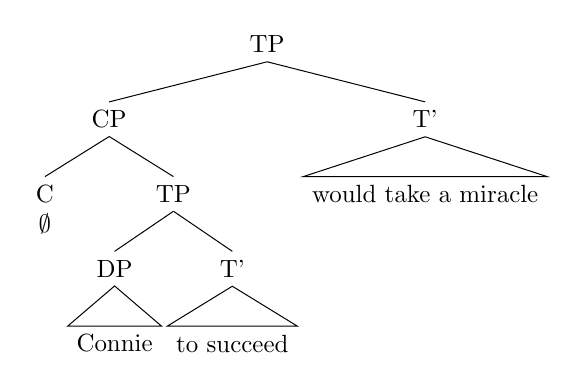
\begin{tikzpicture}[scale=\treeScale, transform shape]
  \tikzset{every tree node/.style={align=center,anchor=north}}
  \Tree
  [.TP
    [.CP
      C\\$\emptyset$
      [.TP
        [.DP
          \edge[roof];
          Connie
        ]
        [.T'
          \edge[roof];
          {to succeed}
        ]
      ]
    ]
    [.T'
      \edge[roof];
      {would take a miracle}
    ]
  ]
\end{tikzpicture} \\

This sentence is ungrammatical because the determiner phrase ``Connie'' does not
recieve abstract case. The tense feature ``to'' does not provide abstract case
and neither does the empty c head. \\

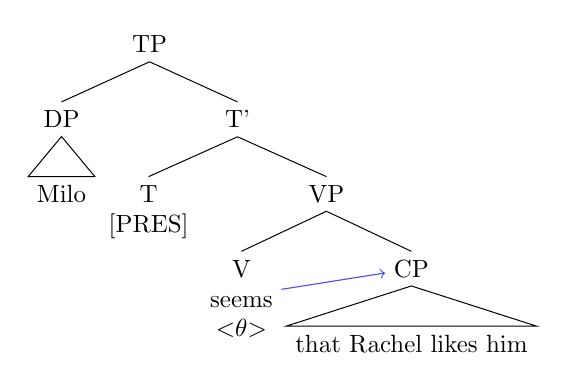
\begin{tikzpicture}[scale=\treeScale, transform shape]
  \tikzset{every tree node/.style={align=center,anchor=north}}
  \Tree
  [.TP
    [.DP
      \edge[roof];
      Milo
    ]
    [.T'
      T\\\feature{PRES}
      [.VP
        \node(V-1){V\\seems\\\rolesOne};
        [.\node(CP-1-1){CP};
          \edge[roof];
          {that Rachel likes him}
        ]
      ]
    ]
  ] 
  \draw[blue, opacity=\rolesOpacity, ->] (V-1) -- (CP-1-1);
\end{tikzpicture} \\

In the example above the constituent ``Milo'' does not receive a theta role as
the verb ``seems'' only has one theta role to assign. Note that the sentence
``It seems that Rachel likes him'' is grammatical as ``It'' does not require a
theta role. \\

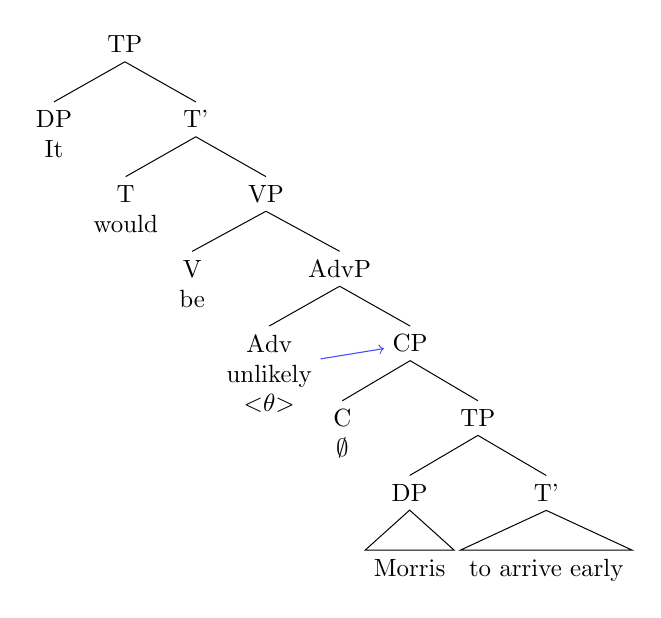
\begin{tikzpicture}[scale=\treeScale, transform shape]
  \tikzset{every tree node/.style={align=center,anchor=north}}
  \Tree
  [.TP
    DP\\{It}
    [.T'
      T\\would
      [.VP
        V\\be
        [.AdvP
          \node(ADV-1-1){Adv\\unlikely\\\rolesOne};
          [.\node(CP-1-1){CP};
            C\\$\emptyset$
            [.TP
              [.DP
                \edge[roof];
                Morris
              ]
              [.T'
                \edge[roof];
                {to arrive early}
              ]
            ]
          ]
        ]
      ]
    ]
  ]
  \draw[blue, opacity=\rolesOpacity, ->] (ADV-1-1) -- (CP-1-1);
\end{tikzpicture} \\

This sentence is ungrammatical because the determiner phrase ``Morris'' does not
recieve abstract case. The tense feature ``to'' does not provide abstract case
and neither does the empty c head. If the CP node was removed the problem would
not be fixed as adverb phrases do not provide case. \\

\begin{tikzpicture}[scale=\treeScale, transform shape]
  \tikzset{every tree node/.style={align=center,anchor=north}}
  \Tree
  [.TP
    [.DP
      \edge[roof];
      Kia
    ]
    [.T'
      T\\\feature{PRES}
      [.VP
        V\\wants
        [.CP
          C\\$\emptyset$
          [.TP
            DP\\\feature{PRO}
            [.T'
              T\\to
              [.VP
                \node(V-2){V\\appear\\\rolesOne};
                [.\node(CP-2-1){CP};
                  \edge[roof];
                  {that Nora wrote the article}
                ]
              ]
            ]
          ]
        ]
      ]
    ]
  ]
  \draw[blue, opacity=\rolesOpacity, ->] (V-2) -- (CP-2-1);
\end{tikzpicture} \\

In the tree above the null pronoun does not receive a theta role as
the verb ``appear'' only has one theta role to assign. Note that the sentence
``Kia wants it to appear that Nora wrote the article'' is grammatical
as ``It'' does not require a theta role.

\newpage

\section{Expect vs Convince}

I'm going to solve this assignment with backwards induction, like a Sudoku
puzzle. Examples (11)-(20) give enough data to test various hypotheses. First
the hypothesis that expect has three theta roles to give is disproven by
sentence (15). Sentence (15), ``\constituent{DP}{Maya} expected \constituent{DP}{the children}
\constituent{CP}{that they would leave}'', is ungrammatical because our
hypothesis is wrong, expect does not have three theta roles to give. Next we can
assume expect has two theta roles to give. This is backed up by sentences
(11), (17), and (19):
\begin{itemize}
\item \constituent{DP}{Maya} expected \constituent{CP}{that the children would leave}
\item \constituent{DP}{Maya} expected \constituent{CP}{it to be raining}
\item \constituent{DP}{Maya} expected \constituent{CP}{there to be food on the table}
\end{itemize}
Thus we can find a tree structure that satisfies the theta criterion: \\

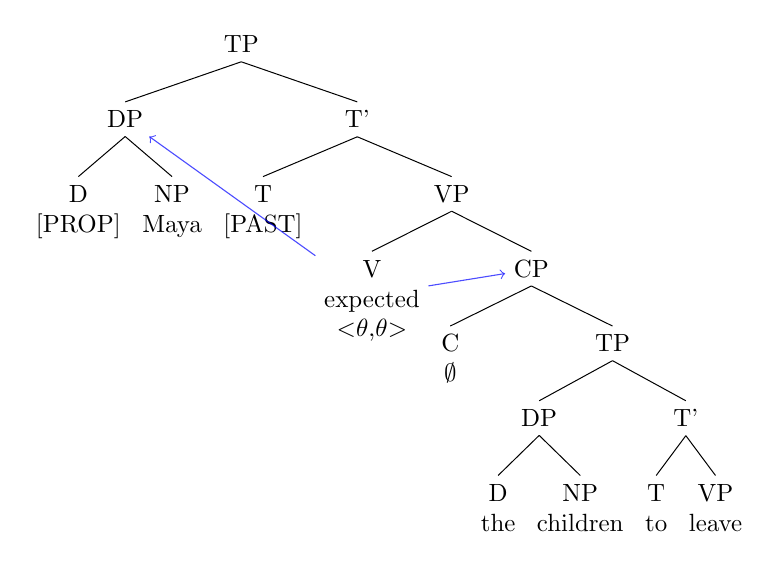
\begin{tikzpicture}[scale=\treeScale, transform shape]
  \tikzset{every tree node/.style={align=center,anchor=north}}
  \Tree
  [.TP
    [.\node(DP-1-1){DP};
      D\\\feature{PROP}
      NP\\Maya
    ]
    [.T'
      T\\\feature{PAST}
      [.VP
        \node(V-1){V\\expected\\\rolesTwo};
        [.\node(CP-1-1){CP};
          C\\$\emptyset$
          [.TP
            [.DP
              D\\the
              NP\\children
            ]
            [.T'
              T\\to
              VP\\leave
            ]
          ]
        ]
      ]
    ]
  ]
  \draw[blue, opacity=\rolesOpacity, ->] (V-1) -- (DP-1-1);
  \draw[blue, opacity=\rolesOpacity, ->] (V-1) -- (CP-1-1);
\end{tikzpicture}

An entirely similar method can be used to show that convince requires three
theta roles: \\

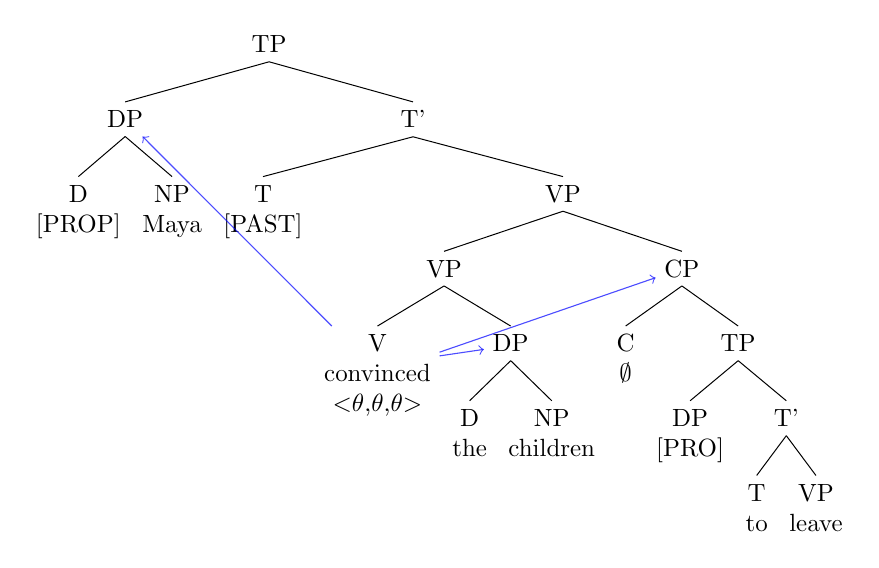
\begin{tikzpicture}[scale=\treeScale, transform shape]
  \tikzset{every tree node/.style={align=center,anchor=north}}
  \Tree
  [.TP
    [.\node(DP-1-1){DP};
      D\\\feature{PROP}
      NP\\Maya
    ]
    [.T'
      T\\\feature{PAST}
      [.VP
        [.VP
          \node(V-1){V\\convinced\\\rolesThree};
          [.\node(DP-1-2){DP};
            D\\the
            NP\\children
          ]
        ]
        [.\node(CP-1-1){CP};
          C\\$\emptyset$
          [.TP
            DP\\\feature{PRO}
            [.T'
              T\\to
              VP\\leave
            ]
          ]
        ]
      ]
    ]
  ]
  \draw[blue, opacity=\rolesOpacity, ->] (V-1) -- (DP-1-1);
  \draw[blue, opacity=\rolesOpacity, ->] (V-1) -- (DP-1-2);
  \draw[blue, opacity=\rolesOpacity, ->] (V-1) -- (CP-1-1);
\end{tikzpicture}

\end{document}

